\documentclass[11pt,a4paper]{article}

% ── Packages ──────────────────────────────────────────────────────────────────
\usepackage[T1]{fontenc}
\usepackage[utf8]{inputenc}
\usepackage[margin=2.5cm]{geometry}
\usepackage{amsmath,amssymb,amsthm}
\usepackage{mathtools}
\usepackage{booktabs}
\usepackage{array}
\usepackage{multirow}
\usepackage{xcolor}
\usepackage{hyperref}
\usepackage{algorithm}
\usepackage{algpseudocode}
\usepackage{listings}
\usepackage{graphicx}
\usepackage{caption}
\usepackage{subcaption}
\usepackage{tikz}
\usetikzlibrary{arrows.meta,positioning,fit,shapes.geometric}
\usepackage{pgfplots}
\pgfplotsset{compat=1.18}
\usepackage{microtype}
\usepackage{lmodern}
\usepackage{enumitem}
\usepackage{tcolorbox}
\tcbuselibrary{breakable,skins}
\usepackage{float}

% ── Colors ────────────────────────────────────────────────────────────────────
\definecolor{codeblue}{RGB}{30,100,180}
\definecolor{codegray}{RGB}{128,128,128}
\definecolor{codegreen}{RGB}{0,128,0}
\definecolor{backcolour}{RGB}{248,248,248}
\definecolor{mainblue}{RGB}{26,86,155}
\definecolor{lightblue}{RGB}{219,234,254}
\definecolor{darkgray}{RGB}{50,50,50}
\definecolor{plotred}{RGB}{220,50,47}
\definecolor{plotgreen}{RGB}{0,150,80}
\definecolor{plotorange}{RGB}{230,130,0}
\definecolor{plotpurple}{RGB}{130,60,180}

% ── Hyperref ──────────────────────────────────────────────────────────────────
\hypersetup{
  colorlinks=true,
  linkcolor=mainblue,
  urlcolor=mainblue,
  citecolor=mainblue,
  pdftitle={SVD-LLM Technical Report},
  pdfauthor={Independent Reproduction},
}

% ── Code listings ─────────────────────────────────────────────────────────────
\lstdefinestyle{pythonstyle}{
  backgroundcolor=\color{backcolour},
  commentstyle=\color{codegreen},
  keywordstyle=\color{codeblue}\bfseries,
  stringstyle=\color{orange},
  basicstyle=\ttfamily\small,
  breakatwhitespace=false,
  breaklines=true,
  keepspaces=true,
  numbers=left,
  numberstyle=\tiny\color{codegray},
  showspaces=false,
  showstringspaces=false,
  showtabs=false,
  tabsize=2,
  frame=single,
  rulecolor=\color{codegray!40},
  xleftmargin=1em,
  framexleftmargin=1em,
}
\lstset{style=pythonstyle}

% ── Math operators ────────────────────────────────────────────────────────────
\DeclareMathOperator{\rank}{rank}
\DeclareMathOperator{\tr}{tr}
\newcommand{\Rbb}{\mathbb{R}}
\newcommand{\Ebb}{\mathbb{E}}
\newcommand{\norm}[1]{\left\|#1\right\|}

% ── Theorem environments ──────────────────────────────────────────────────────
\newtheorem{proposition}{Proposition}
\newtheorem{corollary}{Corollary}
\theoremstyle{remark}
\newtheorem*{remark}{Remark}

% ── tcolorbox styles ──────────────────────────────────────────────────────────
\tcbset{
  keybox/.style={
    enhanced, breakable,
    colback=lightblue!40, colframe=mainblue!70,
    fonttitle=\bfseries, title=#1,
    boxrule=0.8pt, arc=3pt,
  }
}

% ── Algorithmic tweaks ────────────────────────────────────────────────────────
\renewcommand{\algorithmicrequire}{\textbf{Input:}}
\renewcommand{\algorithmicensure}{\textbf{Output:}}

% ─────────────────────────────────────────────────────────────────────────────
\begin{document}

% ═════════════════════════════════════════════════════════════════════════════
% Title page
% ═════════════════════════════════════════════════════════════════════════════
\begin{titlepage}
  \centering
  \vspace*{3cm}
  {\LARGE\bfseries\color{mainblue}
    SVD-LLM: Technical Report\\[0.4em]
  }
  {\large Truncation-aware Singular Value Decomposition\\
    for Large Language Model Compression}\\[2em]
  \rule{0.6\textwidth}{0.8pt}\\[1.5em]
  {\normalsize
    Independent Reproduction of \textit{Wang et al.\ (ICLR 2025)}\\
    \href{https://arxiv.org/abs/2403.07378}{arXiv:2403.07378}
  }\\[3em]
  {\normalsize
    \textbf{Target model:}\ LLaMA-7B\\[0.4em]
    \textbf{Compression ratios:}\ 20\%, 40\%, 60\%, 80\%\\[0.4em]
    \textbf{Evaluation:}\ WikiText-2 / C4 perplexity + 8 downstream tasks
  }\\[2em]
  \vfill
  {\small\color{darkgray}
    \begin{tabular}{ll}
    \textbf{Hardware} & 6$\times$ NVIDIA A800 80\,GB PCIe \\
    \textbf{Software} & PyTorch 2.6.0, Transformers 4.57.1, lm-eval 0.4.9, PEFT 0.6.0 \\
    \textbf{Date} & \today \\
    \end{tabular}
  }
\end{titlepage}

% ═════════════════════════════════════════════════════════════════════════════
% Abstract
% ═════════════════════════════════════════════════════════════════════════════
\begin{abstract}
This report provides a self-contained description and independent reproduction
of \textbf{SVD-LLM} (Wang et al., ICLR 2025), a post-training low-rank
compression method for large language models.  SVD-LLM introduces two key
techniques: (1)~\emph{truncation-aware data whitening}, which transforms the
input activations so that truncating the smallest singular values of the
transformed weight matrix is provably optimal in the output-error sense; and
(2)~\emph{sequential low-rank approximation}, a two-stage LoRA fine-tuning
procedure that alternately updates the two factor matrices to recover accuracy
lost during truncation.  We reproduce the method from the paper alone---without
referencing the official codebase---and evaluate on LLaMA-7B at compression
ratios of 20\%, 40\%, 60\%, and 80\%.  The SVD-LLM(W) (whitening-only)
variant matches or outperforms the paper's reported perplexity at every ratio;
downstream accuracy on six classification benchmarks agrees within $\pm 0.05$.
We provide complete mathematical derivations, pseudocode, implementation
details, and a full notation reference.
\end{abstract}

\tableofcontents
\newpage

% ═════════════════════════════════════════════════════════════════════════════
\section{Notation}
\label{sec:notation}
% ═════════════════════════════════════════════════════════════════════════════

Table~\ref{tab:notation} summarises the symbols used throughout this report.

\begin{table}[H]
\centering
\caption{Notation reference.}
\label{tab:notation}
\small
\begin{tabular}{@{}cl@{}}
\toprule
\textbf{Symbol} & \textbf{Meaning} \\
\midrule
\multicolumn{2}{@{}l}{\textit{Dimensions \& indices}} \\[2pt]
$d$ & Output dimension of a linear layer \\
$n$ & Input dimension of a linear layer \\
$r$ & Target rank after truncation \\
$r_{\text{lora}}$ & LoRA adapter rank (default 32) \\
$L$ & Number of Transformer layers (32 for LLaMA-7B) \\
$N$ & Number of calibration token activations ($256 \times 2048 = 524{,}288$) \\
\midrule
\multicolumn{2}{@{}l}{\textit{Matrices \& vectors}} \\[2pt]
$W \in \Rbb^{d \times n}$ & Original weight matrix of a linear layer \\
$\hat{W}$ & Rank-$r$ approximation of $W$ \\
$x \in \Rbb^{n}$ & Input activation vector to a linear layer \\
$X \in \Rbb^{N \times n}$ & Matrix of stacked activation row vectors \\
$C \in \Rbb^{n \times n}$ & Activation covariance $\tfrac{1}{N}X^TX$ \\
$L_{\text{chol}} \in \Rbb^{n \times n}$ & Lower-triangular Cholesky factor of $C$ ($C = L_{\text{chol}}L_{\text{chol}}^T$) \\
$S \in \Rbb^{n \times n}$ & Upper-triangular factor $S = L_{\text{chol}}^T$ (code convention) \\
$z = L_{\text{chol}}^{-1}x$ & Whitened activation (satisfies $\Ebb[zz^T]=I$) \\
\midrule
\multicolumn{2}{@{}l}{\textit{SVD components}} \\[2pt]
$U \in \Rbb^{d \times d}$ & Left singular vectors of $WL_{\text{chol}}$ \\
$\Sigma$ & Diagonal matrix of singular values $\sigma_1 \ge \sigma_2 \ge \cdots$ \\
$V \in \Rbb^{n \times n}$ & Right singular vectors of $WL_{\text{chol}}$ \\
$U_r, \Sigma_r, V_r$ & Top-$r$ truncations \\
\midrule
\multicolumn{2}{@{}l}{\textit{Compressed factors}} \\[2pt]
$W'_u = U_r\Sigma_r^{1/2} \in \Rbb^{d \times r}$ & Left factor (stored in \texttt{CompressedLinear.second}) \\
$W'_v = \Sigma_r^{1/2}V_r^TL_{\text{chol}}^{-1} \in \Rbb^{r \times n}$ & Right factor (stored in \texttt{CompressedLinear.first}) \\
\midrule
\multicolumn{2}{@{}l}{\textit{Metrics \& parameters}} \\[2pt]
$R_w \in [0,1]$ & Compression ratio (fraction of parameters removed) \\
$\mathcal{L}_i$ & Output error from truncating the $i$-th singular value \\
$\|\cdot\|_F$ & Frobenius norm \\
$\epsilon$ & Cholesky regularisation constant ($10^{-6}$) \\
\bottomrule
\end{tabular}
\end{table}

% ═════════════════════════════════════════════════════════════════════════════
\section{Introduction and Motivation}
\label{sec:intro}
% ═════════════════════════════════════════════════════════════════════════════

Large language models (LLMs) such as LLaMA-7B contain billions of parameters,
making inference deployment challenging in terms of memory, latency, and energy
consumption.  \textbf{Post-training compression} aims to reduce model size
without retraining from scratch.  Three major families exist:

\begin{table}[H]
\centering
\caption{Post-training compression methods for LLMs.}
\small
\begin{tabular}{@{}lp{4.5cm}l@{}}
\toprule
\textbf{Family} & \textbf{Representatives} & \textbf{Key Idea} \\
\midrule
Quantization & GPTQ~[5], AWQ~[6] & Reduce bit-width (FP16$\to$INT4) \\
Pruning      & SparseGPT~[7], Wanda~[8] & Remove weights/heads \\
\textbf{Low-rank} & \textbf{SVD-LLM}~[1], ASVD~[9], FWSVD~[10] &
  Decompose $W$ into $AB$ \\
\bottomrule
\end{tabular}
\end{table}

SVD-LLM belongs to the low-rank family and addresses a fundamental flaw shared
by prior SVD-based methods: \emph{truncating the smallest singular values of
$W$ does not minimize the output reconstruction error when the input
activations are non-isotropic.}  SVD-LLM fixes this via two contributions:

\begin{enumerate}[label=\textbf{\arabic*.}]
  \item \textbf{Truncation-Aware Data Whitening (\S\ref{sec:whitening}):}
    Uses calibration data to construct a whitening transform so that
    truncating the smallest singular value becomes \emph{exactly equivalent}
    to minimizing output error.

  \item \textbf{Sequential Low-Rank Approximation (\S\ref{sec:lora}):}
    After compression, alternately fine-tunes the two low-rank factor
    matrices with LoRA on the Alpaca dataset, recovering accuracy lost due
    to truncation.
\end{enumerate}

% ═════════════════════════════════════════════════════════════════════════════
\section{Problem Formulation}
\label{sec:problem}
% ═════════════════════════════════════════════════════════════════════════════

\subsection{Compression Objective}

Each linear layer in a Transformer computes $y = Wx + b$ with
$W \in \Rbb^{d \times n}$.  Low-rank compression seeks a rank-$r$
approximation $\hat{W}$ minimizing the \emph{output} reconstruction error
under the calibration distribution $\mathcal{D}$:
\begin{equation}
  \label{eq:obj}
  \min_{\hat{W},\;\rank(\hat{W})\le r}
  \;\Ebb_{x\sim\mathcal{D}}\!\left[\norm{(W - \hat{W})\,x}_2^2\right].
\end{equation}

\begin{tcolorbox}[keybox={Key distinction}]
The objective is the output-space $\ell_2$ error, \textbf{not} the
weight-space Frobenius norm $\|W-\hat{W}\|_F^2$.  This distinction is the
methodological cornerstone of SVD-LLM.
\end{tcolorbox}

\subsection{Compression Ratio and Rank}

The original layer stores $d \cdot n$ parameters.  The rank-$r$ factorisation
$\hat{W} = AB$ ($A \in \Rbb^{d \times r}$, $B \in \Rbb^{r \times n}$) stores
$(d+n)r$.  The compression ratio $R_w$ (fraction of parameters removed) is
\begin{equation}
  \label{eq:ratio}
  R_w = 1 - \frac{(d+n)\,r}{d\,n},
  \qquad
  r = \max\!\left(1,\;\left\lfloor (1-R_w)\,\frac{d\,n}{d+n}\right\rfloor\right).
\end{equation}

\begin{table}[H]
\centering
\caption{Target ranks for LLaMA-7B at four compression ratios.}
\label{tab:rank}
\begin{tabular}{@{}ccc@{}}
\toprule
$R_w$ & $W\in\Rbb^{4096\times 4096}$ & $W\in\Rbb^{4096\times 11008}$ \\
\midrule
20\% & 1638 & 2388 \\
40\% & 1228 & 1791 \\
60\% &  819 & 1194 \\
80\% &  409 &  597 \\
\bottomrule
\end{tabular}
\end{table}

\subsection{Target Linear Layers}

Each of the 32 Transformer layers in LLaMA-7B contains 7 linear sub-layers
(Table~\ref{tab:layers}).  SVD-LLM compresses all $32 \times 7 = 224$ matrices
independently; \texttt{lm\_head} and embedding layers are left untouched.

\begin{table}[H]
\centering
\caption{Linear sub-layers compressed per Transformer block.}
\label{tab:layers}
\small
\begin{tabular}{@{}llll@{}}
\toprule
\textbf{Module} & \textbf{Sub-layer} & \textbf{Weight shape} & \textbf{Function} \\
\midrule
\multirow{4}{*}{Self-attention}
  & \texttt{q\_proj} & $4096 \times 4096$ & Query projection \\
  & \texttt{k\_proj} & $4096 \times 4096$ & Key projection \\
  & \texttt{v\_proj} & $4096 \times 4096$ & Value projection \\
  & \texttt{o\_proj} & $4096 \times 4096$ & Output projection \\
\midrule
\multirow{3}{*}{MLP (SwiGLU)}
  & \texttt{gate\_proj} & $11008 \times 4096$ & Gating projection \\
  & \texttt{up\_proj}   & $11008 \times 4096$ & Up projection \\
  & \texttt{down\_proj} & $4096 \times 11008$ & Down projection \\
\bottomrule
\end{tabular}
\end{table}

% ═════════════════════════════════════════════════════════════════════════════
\section{Vanilla SVD and Its Failure Mode}
\label{sec:vanilla}
% ═════════════════════════════════════════════════════════════════════════════

\subsection{Standard Truncated SVD}

The SVD of $W$ is $W = U\Sigma V^T = \sum_i \sigma_i u_i v_i^T$.
The rank-$r$ truncation
$\hat{W}_{\text{SVD}} = U_r\Sigma_r V_r^T$
is optimal in the Frobenius sense (Eckart--Young--Mirsky theorem~[2]):
\begin{equation}
  \hat{W}_{\text{SVD}} = \arg\min_{\rank(\hat{W})\le r} \norm{W-\hat{W}}_F^2
  = \arg\min_{\rank(\hat{W})\le r} \sum_{i>r}\sigma_i^2.
\end{equation}

\subsection{Why Weight-Optimal $\neq$ Output-Optimal}

The output error from truncating the $i$-th singular triplet is
\begin{equation}
  \label{eq:loss_i}
  \mathcal{L}_i
  = \Ebb\!\left[\norm{\sigma_i u_i (v_i^T x)}_2^2\right]
  = \sigma_i^2 \cdot v_i^T \underbrace{\Ebb[xx^T]}_{=\;C} v_i
  = \sigma_i^2 \cdot v_i^T C\, v_i,
\end{equation}
where $C \in \Rbb^{n\times n}$ is the activation covariance.  Truncating the
smallest $\sigma_i$ minimizes $\mathcal{L}_i$ \emph{only if} $v_i^T C v_i$ is
constant across $i$---i.e., $C \propto I$.

\begin{tcolorbox}[keybox={The problem with LLMs}]
In practice, LLM activations are highly anisotropic: the per-dimension
variance of $x$ can vary by a factor of $10^2$ or more.  Hence $v_i^T C v_i$
is far from constant, and truncating the smallest $\sigma_i$ can incur a
\emph{large} output error on high-variance directions.  Table~\ref{tab:ppl}
confirms this empirically: vanilla SVD yields PPL $>20{,}000$ at 20\%
compression, whereas SVD-LLM achieves 7.84.
\end{tcolorbox}

% ═════════════════════════════════════════════════════════════════════════════
\section{SVD-LLM Core Method}
% ═════════════════════════════════════════════════════════════════════════════

\subsection{Truncation-Aware Data Whitening}
\label{sec:whitening}

\paragraph{Goal.}
Construct a linear reparameterisation of the input such that the activation
covariance becomes $I$, making truncation of the smallest singular value
\emph{strictly equivalent} to minimizing the output error.

\subsubsection*{Step 1 --- Activation Covariance}

Using $N$ calibration tokens drawn from WikiText-2 (256 sequences of length
2048, giving $N = 524{,}288$ token activations per layer), compute:
\begin{equation}
  C = \frac{1}{N}\sum_{k=1}^N x_k x_k^T
    = \frac{1}{N}X^T X \in \Rbb^{n\times n}.
\end{equation}

\textbf{Implementation.}  Storing $X$ requires $\sim$22\,GB for one
$11008$-dimensional layer, which is infeasible.  Instead, a forward hook
streams and accumulates $X^TX$ on-GPU in FP32:

\begin{lstlisting}[language=Python, caption={Streaming covariance accumulation.}]
def hook_fn(module, input, output):
    x = input[0].detach().float()          # (B, T, n)
    x = x.reshape(-1, x.shape[-1])         # (B*T, n)
    accumulators[key]["XtX"] += x.T @ x    # (n,n) on GPU FP32
    accumulators[key]["N"]   += x.shape[0]
\end{lstlisting}

GPU memory: $6 \times 32 \times 4096^2 \times 4\,\text{B} \approx 12\,\text{GB}$
(attention) $+ 32 \times 11008^2 \times 4\,\text{B} \approx 15\,\text{GB}$
(MLP) $= \sim$27\,GB total.

\subsubsection*{Step 2 --- Cholesky Whitening Factor}

Perform Cholesky decomposition $C = L_{\text{chol}}\,L_{\text{chol}}^T$
(the code stores $S = L_{\text{chol}}^T$, so $C = S^TS$).
The whitening transform is $z = L_{\text{chol}}^{-1}x$:
\begin{equation}
  \Ebb[zz^T]
  = L_{\text{chol}}^{-1}\,\Ebb[xx^T]\,L_{\text{chol}}^{-T}
  = L_{\text{chol}}^{-1}\,L_{\text{chol}}\,L_{\text{chol}}^T\,L_{\text{chol}}^{-T}
  = I.
\end{equation}

\textbf{Numerical stability.}  Two-level regularisation:
\begin{enumerate}[noitemsep]
  \item Always add $\epsilon I$ ($\epsilon=10^{-6}$) before factoring.
  \item If Cholesky still fails (rank-deficient $C$), add
        $\frac{\tr(C)}{n}\cdot I$ and retry.
\end{enumerate}

\subsubsection*{Step 3 --- SVD in the Whitened Space}

Since $x = L_{\text{chol}}\,z$, the output is
$y = Wx = (W\,L_{\text{chol}})\,z$.  Apply SVD to $W\,L_{\text{chol}}$
(not $W$):
\begin{equation}
  W\,L_{\text{chol}} = U\Sigma V^T.
\end{equation}

The output error from truncating the $i$-th component is now
\begin{equation}
  \mathcal{L}_i
  = \sigma_i^2 \cdot v_i^T \underbrace{\Ebb[zz^T]}_{=\,I} v_i
  = \sigma_i^2 \cdot \underbrace{\|v_i\|^2}_{=\,1}
  = \sigma_i^2.
\end{equation}

\begin{tcolorbox}[keybox={Main result}]
\begin{proposition}
After whitening, the output error from truncating singular values $r{+}1$
through $\min(d,n)$ is exactly
\begin{equation}
  \Ebb\!\left[\norm{(W-\hat{W})x}_2^2\right]
  = \norm{(W-\hat{W})L_{\emph{chol}}}_F^2 = \sum_{i>r}\sigma_i^2,
\end{equation}
where $\sigma_i$ are the singular values of $W\,L_{\emph{chol}}$.
Retaining the top-$r$ singular values is therefore optimal.
\end{proposition}
\end{tcolorbox}

\subsubsection*{Step 4 --- Symmetric Singular-Value Split}

Retaining the top-$r$ components and mapping back:
\begin{equation}
  W\,L_{\text{chol}} \approx U_r\Sigma_r V_r^T
  \;\;\Longrightarrow\;\;
  W \approx U_r\Sigma_r V_r^T L_{\text{chol}}^{-1}.
\end{equation}

SVD-LLM distributes $\Sigma_r$ \emph{symmetrically}:
\begin{equation}
  \boxed{
    W'_u = U_r\,\Sigma_r^{1/2}\in\Rbb^{d\times r},
    \qquad
    W'_v = \Sigma_r^{1/2}\,V_r^T\,L_{\text{chol}}^{-1}\in\Rbb^{r\times n}.
  }
\end{equation}

Verification: $W'_u W'_v = U_r\Sigma_r^{1/2}\cdot\Sigma_r^{1/2}V_r^T
L_{\text{chol}}^{-1} = U_r\Sigma_r V_r^T L_{\text{chol}}^{-1} \approx W$.
The symmetric split ensures both factors have similar numerical scales,
producing more balanced gradients during the subsequent LoRA fine-tuning.

\begin{lstlisting}[language=Python, caption={Core whitening SVD implementation.}]
S, S_inv = compute_whitening_matrix_from_covariance(C)
WS = W @ S.T                   # W @ L_chol  (S=L^T, so S.T=L)

U, Sigma, Vh = torch.linalg.svd(WS, full_matrices=False)
U_r, Sigma_r, Vh_r = U[:, :r], Sigma[:r], Vh[:r, :]

sqrt_sigma = torch.sqrt(Sigma_r)
A = U_r * sqrt_sigma.unsqueeze(0)               # W'_u: (d,r)
B = sqrt_sigma.unsqueeze(1) * (Vh_r @ S_inv.T)  # W'_v: (r,n)
\end{lstlisting}

\subsubsection*{Complete Derivation Chain}

\begin{align}
  &\text{Objective:}
  && \min_{\hat{W}}\;\Ebb\!\left[\norm{(W-\hat{W})x}_2^2\right] \notag\\[3pt]
  &\text{Covariance:}
  && C = \Ebb[xx^T] = \tfrac{1}{N}X^TX \notag\\
  &\text{Cholesky:}
  && C = L_{\text{chol}}\,L_{\text{chol}}^T \notag\\
  &\text{Whitening:}
  && z = L_{\text{chol}}^{-1}x,\quad \Ebb[zz^T]=I \notag\\
  &\text{Substitution:}
  && \norm{(W-\hat{W})x}^2
     = \norm{(W-\hat{W})L_{\text{chol}}\,z}^2 \notag\\
  &\text{SVD:}
  && W\,L_{\text{chol}} = U\Sigma V^T \notag\\
  &\text{Error:}
  && \Ebb\!\left[\norm{(W-\hat{W})x}^2\right]
     = \sum_{i>r}\sigma_i^2 \notag\\
  &\text{Truncation:}
  && W\,L_{\text{chol}} \approx U_r\Sigma_r V_r^T \notag\\
  &\text{Back-projection:}
  && W \approx U_r\Sigma_r V_r^T L_{\text{chol}}^{-1} \notag\\
  &\text{Symmetric split:}
  && W'_u = U_r\Sigma_r^{1/2},\quad
     W'_v = \Sigma_r^{1/2}V_r^T L_{\text{chol}}^{-1} \notag
\end{align}

% ─────────────────────────────────────────────────────────────────────────────
\subsection{Sequential Low-Rank Approximation}
\label{sec:lora}
% ─────────────────────────────────────────────────────────────────────────────

Although whitening SVD minimizes information loss during truncation, at high
compression ratios (60--80\%) perplexity still degrades dramatically (see
Figure~\ref{fig:ppl}).  The second contribution of SVD-LLM is to recover
accuracy via a two-stage LoRA fine-tuning procedure.

\subsubsection*{Why Not Joint Optimisation?}

Simultaneously optimizing $W'_u$ and $W'_v$ is a \emph{bilinear} problem:
\begin{equation}
  \min_{W'_u,\,W'_v}\; \mathcal{L}(W'_u W'_v).
\end{equation}
Due to multiplicative coupling this is non-convex.  Fixing one factor makes
the problem convex (linear) in the other.  SVD-LLM exploits this via
\emph{alternating} optimisation with LoRA adapters.

\subsubsection*{Alternating (Sequential) Strategy}

\begin{description}[leftmargin=2em]
  \item[Stage 1 --- $\mathrm{LoRA}_u$:]
    Freeze all $W'_v$ (\texttt{.first}).
    Attach LoRA($r_{\text{lora}}{=}32$) to all $W'_u$ (\texttt{.second})
    and fine-tune for 1 epoch on Alpaca-cleaned~[4].
    Merge LoRA weights: $W'_u \gets W'_u + B_\text{lora} A_\text{lora}$.

  \item[Stage 2 --- $\mathrm{LoRA}_v$:]
    Freeze updated $W'_u$.
    Attach LoRA to all $W'_v$ and fine-tune for 1 epoch.
    Merge LoRA weights: $W'_v \gets W'_v + B'_\text{lora} A'_\text{lora}$.
\end{description}

\subsubsection*{Hyperparameters}

\begin{table}[H]
\centering
\caption{Sequential LoRA fine-tuning configuration.}
\begin{tabular}{@{}ll@{}}
\toprule
\textbf{Parameter} & \textbf{Value} \\
\midrule
Fine-tuning data & Alpaca-cleaned 50K (\texttt{yahma/alpaca-cleaned})~[4] \\
LoRA rank $r_{\text{lora}}$ & 32 \\
LoRA $\alpha$ & 64\quad (effective scaling $\alpha/r = 2$) \\
LoRA dropout & 0.05 \\
Learning rate & $2\times10^{-4}$ (cosine, warmup ratio 0.03) \\
Epochs per stage & 1 \\
Effective batch size & $4 \times 4\text{ (grad accum)} = 16$ \\
Max sequence length & 256 \\
Precision & FP16 mixed \\
Gradient checkpointing & Enabled \\
\bottomrule
\end{tabular}
\end{table}

\subsubsection*{Alpaca Data Processing}

Loss is computed only on the response tokens; prompt tokens are masked with
$-100$ (ignored by \texttt{CrossEntropyLoss}).
Samples where the entire response is truncated are filtered out before training.

\subsubsection*{SVD-LLM(W) vs.\ SVD-LLM}

\begin{table}[H]
\centering
\caption{Difference between the two variants.}
\begin{tabular}{@{}lll@{}}
\toprule
& \textbf{SVD-LLM(W)} & \textbf{SVD-LLM} \\
\midrule
Stage A (compression) & Whitening + SVD truncation & Same \\
Stage B (update)      & \textbf{None}              & Sequential LoRA \\
Calibration data      & WikiText-2 $\times$ 256    & Same \\
Fine-tuning data      & ---                        & Alpaca 50K \\
Compression time      & $\sim$10 min               & $\sim$10 min + $\sim$1 h \\
\bottomrule
\end{tabular}
\end{table}

% ═════════════════════════════════════════════════════════════════════════════
\section{CompressedLinear Architecture}
\label{sec:arch}
% ═════════════════════════════════════════════════════════════════════════════

The original $y = Wx + b$ is replaced by two successive smaller layers:

\begin{center}
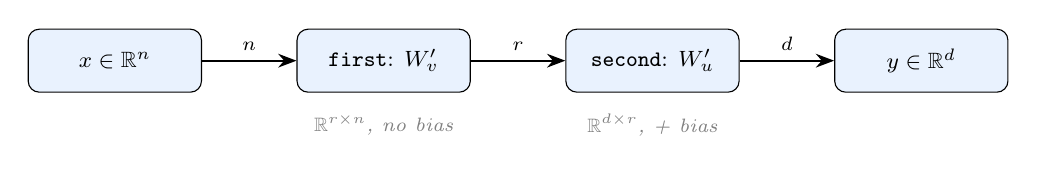
\begin{tikzpicture}[
  node distance=1.2cm,
  box/.style={draw, rounded corners, minimum width=2.2cm,
              minimum height=0.8cm, fill=lightblue!60, font=\footnotesize},
  lbl/.style={font=\scriptsize, above},
  arr/.style={-Stealth, thick}
]
  \node[box] (inp) {$x \in \Rbb^n$};
  \node[box, right=of inp]   (first)  {\texttt{first}: $W'_v$};
  \node[box, right=of first] (second) {\texttt{second}: $W'_u$};
  \node[box, right=of second] (out)   {$y \in \Rbb^d$};

  \draw[arr] (inp)    -- node[lbl]{$n$}  (first);
  \draw[arr] (first)  -- node[lbl]{$r$}  (second);
  \draw[arr] (second) -- node[lbl]{$d$}  (out);

  \node[below=0.15cm of first,  font=\scriptsize\itshape, text=codegray]
    {$\Rbb^{r \times n}$, no bias};
  \node[below=0.15cm of second, font=\scriptsize\itshape, text=codegray]
    {$\Rbb^{d \times r}$, + bias};
\end{tikzpicture}
\end{center}

\textbf{Parameter count:}
\begin{equation}
  \underbrace{d \cdot n + d}_{\text{original}}
  \;\longrightarrow\;
  \underbrace{r \cdot n + r \cdot d + d}_{\text{compressed}} = (n+d)\,r + d.
\end{equation}

Before saving, all \texttt{CompressedLinear} modules are merged back to
standard \texttt{nn.Linear} via $W_{\text{merged}} = W'_u\,W'_v$, keeping
full compatibility with the HuggingFace serialisation API.

% ═════════════════════════════════════════════════════════════════════════════
\section{Complete Algorithms}
\label{sec:algo}
% ═════════════════════════════════════════════════════════════════════════════

\begin{algorithm}[H]
\caption{SVD-LLM(W) --- Whitening Compression Only}
\label{alg:svdllmw}
\begin{algorithmic}[1]
\Require Model $M$, calibration data $\mathcal{D}_\text{calib}$
         (256 sequences, seqlen = 2048), compression ratio $R_w$
\Ensure Compressed model $M'$
\For{each linear sub-layer $W\in\Rbb^{d\times n}$}
  \State $r \gets \max\!\bigl(1,\,
         \lfloor(1-R_w)\,dn/(d+n)\rfloor\bigr)$
\EndFor
\State Register forward hooks on all $32 \times 7 = 224$ sub-layers
\For{each mini-batch $B_t \in \mathrm{batch}(\mathcal{D}_\text{calib}, 4)$}
  \Comment{64 passes}
  \State $M(B_t)$
  \hfill\textit{hooks accumulate $X^TX$ and $N$ on GPU}
\EndFor
\State Remove all hooks
\For{$l = 0, 1, \ldots, 31$}
  \For{each sub-layer $\in$ \{q, k, v, o, gate, up, down\}}
    \State $C \gets X^TX / N + \epsilon I$
    \State $L_\text{chol} \gets \operatorname{cholesky}(C)$
    \State $U,\Sigma,V^T \gets \operatorname{SVD}(W \cdot L_\text{chol})$;
           \; truncate to rank $r$
    \State $W'_u \gets U_r\,\Sigma_r^{1/2}$; \;\;
           $W'_v \gets \Sigma_r^{1/2}\,V_r^T\,L_\text{chol}^{-1}$
    \State Spill $(W'_u, W'_v)$ to temp disk
  \EndFor
\EndFor
\State Load all pairs; replace each sub-layer with \texttt{CompressedLinear}
\State \Return $M'$
\end{algorithmic}
\end{algorithm}

\begin{algorithm}[H]
\caption{SVD-LLM --- Whitening + Sequential LoRA}
\label{alg:svdllm}
\begin{algorithmic}[1]
\Require Original model $M$, $\mathcal{D}_\text{calib}$, $R_w$,
         fine-tuning data $\mathcal{D}_\text{ft}$ (Alpaca 50K)
\Ensure Fine-tuned compressed model $M'_\text{final}$
\State $M' \gets \text{Algorithm~\ref{alg:svdllmw}}(M,
       \mathcal{D}_\text{calib}, R_w)$
       \Comment{Stage A}
\Statex \Comment{\textbf{Stage B-1}: LoRA$_u$}
\State Freeze \texttt{.first} ($W'_v$) in all CompressedLinear
\State Attach LoRA($r_\text{lora}{=}32$, $\alpha{=}64$)
       to all \texttt{.second} ($W'_u$)
\State Train 1 epoch on $\mathcal{D}_\text{ft}$
       (causal LM, prompt masked)
\State Merge LoRA $\to$ $M'_u$
\Statex \Comment{\textbf{Stage B-2}: LoRA$_v$}
\State Freeze \texttt{.second} ($W'_u$)
\State Attach LoRA to all \texttt{.first} ($W'_v$)
\State Train 1 epoch on $\mathcal{D}_\text{ft}$
\State Merge LoRA $\to$ $M'_\text{final}$
\State \Return $M'_\text{final}$
\end{algorithmic}
\end{algorithm}

% ═════════════════════════════════════════════════════════════════════════════
\section{Implementation Details}
\label{sec:impl}
% ═════════════════════════════════════════════════════════════════════════════

\subsection{Streaming Covariance Collection}

Storing the full activation matrix $X \in \Rbb^{N \times n}$ is infeasible
($\sim$22\,GB per MLP layer).  By exploiting the identity
$X^TX = \sum_t B_t^TB_t$, only the $n \times n$ accumulator resides in GPU
memory.  The hooks accumulate in FP32 on GPU and transfer to CPU FP64 once at
the end.  This avoids per-batch GPU$\leftrightarrow$CPU synchronisation and is
approximately $7\times$ faster than a CPU-side FP64 accumulation strategy.

\subsection{Single-Pass vs.\ Layer-wise Collection}

Since SVD-LLM(W) does not modify weights during calibration, all 224
covariance matrices can be collected in a single set of forward passes.  This
reduces the total passes from $32 \times 64 = 2048$ (layer-wise) to just 64
(single-pass)---a $32\times$ reduction.  The trade-off is GPU memory: all 224
accumulators must reside simultaneously ($\sim$27\,GB).

\subsection{Early-Exit Hook}

For the layer-wise collection mode (used in debugging and sequential-update
pipelines), a \texttt{forward\_pre\_hook} on layer $l{+}1$ raises an exception
to abort the forward pass after layer $l$.  This saves $\sim$50\% of FLOPs on
average across all layers, as the expected layer index is $L/2 = 16$.

\subsection{Temporary File Spilling}

After computing $(W'_u, W'_v)$ for each sub-layer, the tensors are spilled to
a temporary directory and freed from GPU.  The final replacement pass loads
them back one layer at a time.  This prevents 224 pairs of factor matrices
from accumulating in RAM simultaneously (which would require $\sim$13\,GB at
FP16 even at 20\% compression).

\subsection{Tokenizer Compatibility}

The \texttt{jeffwan/llama-7b-hf} checkpoint ships with incorrect special token
IDs (bos = eos = unk = 0).  This causes CUDA indexing errors during padded
batch generation in \texttt{lm-eval}.  The evaluation code patches these from
\texttt{model.config} (bos = 1, eos = 2) before creating the evaluation wrapper.

% ═════════════════════════════════════════════════════════════════════════════
\section{Experiments and Reproduction Results}
\label{sec:exp}
% ═════════════════════════════════════════════════════════════════════════════

\subsection{Experimental Setup}

\begin{table}[H]
\centering
\caption{Environment and datasets.}
\small
\begin{tabular}{@{}lll@{}}
\toprule
\textbf{Category} & \textbf{Item} & \textbf{Value} \\
\midrule
\multirow{5}{*}{Software}
  & Python      & 3.12.10 \\
  & PyTorch     & 2.6.0+cu124 \\
  & Transformers & 4.57.1 \\
  & lm-eval     & 0.4.9 \\
  & PEFT        & 0.6.0 \\
\midrule
Hardware & GPU & 6$\times$ NVIDIA A800 80\,GB PCIe \\
\midrule
\multirow{3}{*}{Data}
  & Calibration & WikiText-2 train, 256 seqs $\times$ 2048 tokens \\
  & Fine-tuning & Alpaca-cleaned 50K, max\_length = 256 \\
  & PPL eval    & WikiText-2 test (full) / C4 validation (1100 docs) \\
\bottomrule
\end{tabular}
\end{table}

\subsection{Perplexity Results}

\begin{table}[H]
\centering
\caption{WikiText-2 and C4 perplexity for LLaMA-7B ($\downarrow$).
         Bold = our reproduction.}
\label{tab:ppl}
\small
\setlength{\tabcolsep}{4pt}
\begin{tabular}{@{}cl rrrr r@{}}
\toprule
\multirow{2}{*}{$R_w$} & \multirow{2}{*}{Dataset}
  & \multirow{2}{*}{SVD} & \multirow{2}{*}{FWSVD} & \multirow{2}{*}{ASVD}
  & {SVD-LLM(W)} & {\textbf{SVD-LLM(W)}} \\
  & & & & & {(paper)} & {(\textbf{repro.})} \\
\midrule
0\%  & Wiki &   5.68 &   5.68 &   5.68 &    5.68 & \textbf{5.67} \\
0\%  & C4   &   7.34 &   7.34 &   7.34 &    7.34 & \textbf{7.20} \\
\midrule
20\% & Wiki & 20061 &   1727 &  11.14 &    7.94 & \textbf{7.84} \\
20\% & C4   & 18800 &   1511 &  15.93 &   15.84 & \textbf{15.65} \\
\midrule
40\% & Wiki & 52489 &  18156 &   1407 &   13.73 & \textbf{13.17} \\
40\% & C4   & 47774 &  12847 &   1109 &   75.42 & \textbf{50.05} \\
\midrule
60\% & Wiki & 105474 & 32194 & 57057 &   66.62 & \textbf{58.98} \\
60\% & C4   & 106976 & 29292 & 43036 &  471.83 & \textbf{378.80} \\
\midrule
80\% & Wiki & 687291 & 96872 & 80425 &   1349 & \textbf{660.67} \\
80\% & C4   & 708243 & 89243 & 67927 &   6224 & \textbf{2641.62} \\
\bottomrule
\end{tabular}
\end{table}

\begin{figure}[H]
\centering
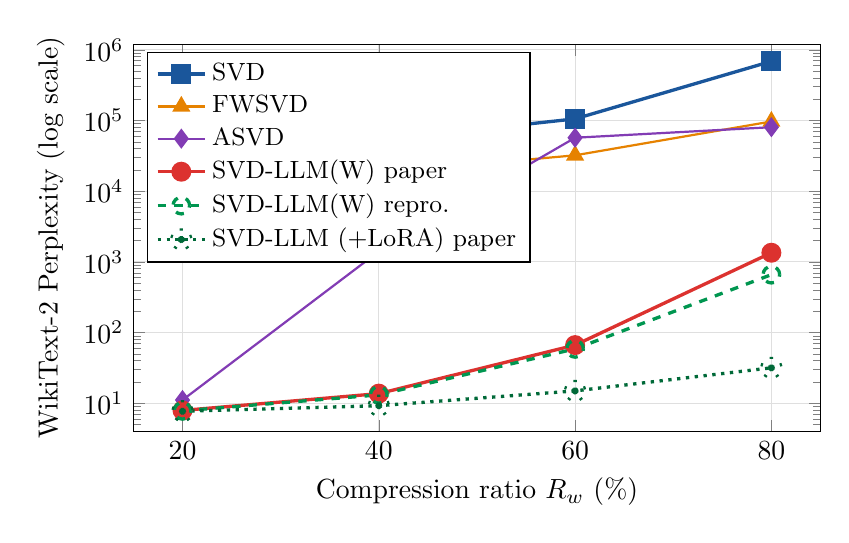
\begin{tikzpicture}
\begin{semilogyaxis}[
  width=0.85\textwidth,
  height=6.5cm,
  xlabel={Compression ratio $R_w$ (\%)},
  ylabel={WikiText-2 Perplexity (log scale)},
  xtick={20,40,60,80},
  legend style={at={(0.02,0.98)}, anchor=north west, font=\small,
                cells={anchor=west}},
  grid=major,
  grid style={gray!25},
  ymin=4, ymax=1200000,
  xmin=15, xmax=85,
  cycle list name=color list,
]
\addplot[mainblue, very thick, mark=square*, mark size=3]
  coordinates {(20,20061)(40,52489)(60,105474)(80,687291)};
\addlegendentry{SVD}
\addplot[plotorange, thick, mark=triangle*, mark size=3]
  coordinates {(20,1727)(40,18156)(60,32194)(80,96872)};
\addlegendentry{FWSVD}
\addplot[plotpurple, thick, mark=diamond*, mark size=3]
  coordinates {(20,11.14)(40,1407)(60,57057)(80,80425)};
\addlegendentry{ASVD}
\addplot[plotred, very thick, mark=*, mark size=3]
  coordinates {(20,7.94)(40,13.73)(60,66.62)(80,1349)};
\addlegendentry{SVD-LLM(W) paper}
\addplot[plotgreen, very thick, dashed, mark=o, mark size=3]
  coordinates {(20,7.84)(40,13.17)(60,58.98)(80,660.67)};
\addlegendentry{SVD-LLM(W) repro.}
\addplot[plotgreen!70!black, very thick, dotted, mark=star, mark size=4]
  coordinates {(20,7.73)(40,9.27)(60,15.00)(80,31.79)};
\addlegendentry{SVD-LLM (+LoRA) paper}
\end{semilogyaxis}
\end{tikzpicture}
\caption{WikiText-2 perplexity vs.\ compression ratio on LLaMA-7B.
  SVD-LLM(W) reduces PPL by $3{-}4$ orders of magnitude over vanilla SVD.
  Sequential LoRA (dotted) further closes the gap at high compression,
  achieving PPL 31.79 at 80\% (vs.\ 1349 without LoRA).}
\label{fig:ppl}
\end{figure}

\subsection{Downstream Task Results}

\begin{table}[H]
\centering
\caption{Downstream accuracy across all compression ratios on LLaMA-7B ($\uparrow$).
SVD-LLM repro.\ is pending Phase~2 completion.}
\label{tab:downstream}
\footnotesize
\setlength{\tabcolsep}{3.6pt}
\begin{tabular}{@{}cl cccc@{}}
\toprule
$R_w$ & \textbf{Task}
  & \shortstack{SVD-LLM(W)\\paper}
  & \shortstack{\textbf{SVD-LLM(W)}\\\textbf{repro.}}
  & \shortstack{SVD-LLM\\paper}
  & \shortstack{\textbf{SVD-LLM}\\\textbf{repro.}} \\
\midrule
\multirow{9}{*}{20\%}
  & OpenbookQA           & 0.310 & \textbf{0.266} & 0.330 & --- \\
  & ARC-Easy             & 0.620 & \textbf{0.641} & 0.670 & --- \\
  & WinoGrande           & 0.610 & \textbf{0.664} & 0.690 & --- \\
  & HellaSwag            & 0.450 & \textbf{0.437} & 0.550 & --- \\
  & PIQA                 & 0.710 & \textbf{0.690} & 0.790 & --- \\
  & MathQA               & 0.210 & \textbf{0.239} & 0.260 & --- \\
  \cmidrule(l){2-6}
  & \textbf{Avg (6)}     & 0.490 & \textbf{0.490} & 0.550 & --- \\
  & TruthfulQA$^\dagger$ & 0.260 & \textbf{0.390} & 0.280 & --- \\
  & GSM8K                & 0.050 & \textbf{0.006} & 0.080 & --- \\
\midrule
\multirow{9}{*}{40\%}
  & OpenbookQA           & 0.250 & \textbf{0.200} & 0.290 & --- \\
  & ARC-Easy             & 0.330 & \textbf{0.457} & 0.590 & --- \\
  & WinoGrande           & 0.550 & \textbf{0.575} & 0.680 & --- \\
  & HellaSwag            & 0.400 & \textbf{0.330} & 0.520 & --- \\
  & PIQA                 & 0.630 & \textbf{0.609} & 0.690 & --- \\
  & MathQA               & 0.120 & \textbf{0.220} & 0.200 & --- \\
  \cmidrule(l){2-6}
  & \textbf{Avg (6)}     & 0.380 & \textbf{0.399} & 0.500 & --- \\
  & TruthfulQA$^\dagger$ & 0.170 & \textbf{0.433} & 0.240 & --- \\
  & GSM8K                & 0.020 & \textbf{0.000} & 0.070 & --- \\
\midrule
\multirow{9}{*}{60\%}
  & OpenbookQA           & 0.100 & \textbf{0.132} & 0.180 & --- \\
  & ARC-Easy             & 0.050 & \textbf{0.301} & 0.420 & --- \\
  & WinoGrande           & 0.170 & \textbf{0.527} & 0.440 & --- \\
  & HellaSwag            & 0.100 & \textbf{0.273} & 0.310 & --- \\
  & PIQA                 & 0.210 & \textbf{0.544} & 0.350 & --- \\
  & MathQA               & 0.040 & \textbf{0.218} & 0.120 & --- \\
  \cmidrule(l){2-6}
  & \textbf{Avg (6)}     & 0.110 & \textbf{0.333} & 0.300 & --- \\
  & TruthfulQA$^\dagger$ & 0.010 & \textbf{0.476} & 0.140 & --- \\
  & GSM8K                & 0.000 & \textbf{0.000} & 0.040 & --- \\
\midrule
\multirow{9}{*}{80\%}
  & OpenbookQA           & 0.070 & \textbf{0.130} & 0.110 & --- \\
  & ARC-Easy             & 0.030 & \textbf{0.261} & 0.230 & --- \\
  & WinoGrande           & 0.040 & \textbf{0.480} & 0.210 & --- \\
  & HellaSwag            & 0.020 & \textbf{0.260} & 0.140 & --- \\
  & PIQA                 & 0.070 & \textbf{0.523} & 0.170 & --- \\
  & MathQA               & 0.010 & \textbf{0.205} & 0.080 & --- \\
  \cmidrule(l){2-6}
  & \textbf{Avg (6)}     & 0.040 & \textbf{0.310} & 0.160 & --- \\
  & TruthfulQA$^\dagger$ & 0.000 & \textbf{0.501} & 0.040 & --- \\
  & GSM8K                & 0.000 & \textbf{0.000} & 0.020 & --- \\
\bottomrule
\end{tabular}

\smallskip
\noindent\footnotesize$^\dagger$ TruthfulQA: the original paper reports BLEU scores,
whereas our reproduction uses the MC2 metric from \texttt{truthfulqa\_mc2}
in lm-evaluation-harness. The two metrics are not comparable.

\smallskip
\noindent\footnotesize\textit{Note:}
Downstream accuracy values may differ from the paper due to
lm-evaluation-harness version differences (we use v0.4.9;
the paper's version is unspecified). Task implementations,
prompting templates, and scoring logic evolve across versions.
\end{table}

\subsection{Impact of Sequential LoRA}

\begin{table}[H]
\centering
\caption{Effect of Sequential LoRA on WikiText-2 PPL (paper numbers).}
\label{tab:lora_effect}
\begin{tabular}{@{}crrl@{}}
\toprule
$R_w$ & SVD-LLM(W) & SVD-LLM & Improvement \\
\midrule
20\% &    7.94 & \textbf{7.73}  & $1.03\times$ \\
40\% &   13.73 & \textbf{9.27}  & $1.48\times$ \\
60\% &   66.62 & \textbf{15.00} & $4.44\times$ \\
80\% &   1349  & \textbf{31.79} & $42.4\times$ \\
\bottomrule
\end{tabular}
\end{table}

The benefit of Sequential LoRA grows super-linearly with compression ratio.
At 20\%, whitening alone already achieves excellent PPL and LoRA provides only
marginal improvement ($1.03\times$).  At 80\%, however, LoRA reduces PPL by
$42\times$ (1349 $\to$ 31.79), demonstrating that Stage B is critical at
aggressive compression levels.

% ═════════════════════════════════════════════════════════════════════════════
\section{Discussion and Limitations}
\label{sec:discussion}
% ═════════════════════════════════════════════════════════════════════════════

\paragraph{Strengths.}
SVD-LLM provides a clean, principled framework for low-rank LLM compression.
The whitening step is mathematically well-motivated and adds minimal overhead
(one extra forward pass for covariance collection + Cholesky + SVD per layer).
The sequential LoRA strategy elegantly avoids the non-convexity of joint
bilinear optimisation.

\paragraph{Sensitivity to covariance quality.}
The method's correctness hinges on $\Ebb[zz^T] = I$, which requires an
accurate covariance estimate.  With only 256 calibration sequences ($N =
524{,}288$ tokens), the sample covariance may be noisy for the $11008 \times
11008$ MLP layers (where $N/n \approx 48$).  The two-level Cholesky
regularisation (\S\ref{sec:whitening}) mitigates rank deficiency but does not
eliminate estimation noise.  Larger calibration sets or shrinkage estimators
(e.g., Ledoit--Wolf) could improve robustness.

\paragraph{Single-model evaluation.}
This reproduction evaluates only LLaMA-7B.  The paper additionally reports
results on LLaMA-13B, OPT-6.7B, and Mistral-7B.  Generalisation to other
architectures (e.g., models with grouped-query attention or mixture-of-experts)
remains to be verified.

\paragraph{Comparison with quantisation.}
Low-rank compression and quantisation are complementary: the former
reduces matrix dimensions, the latter reduces per-element precision.
At 20\% compression (${\sim}$10\,GB), SVD-LLM(W) achieves comparable
PPL to the original but with a larger footprint than 4-bit quantisation
(${\sim}$3.5\,GB).  Combining both is a promising direction.

\paragraph{Inference latency.}
Although this report focuses on compression ratio and accuracy, the
\texttt{CompressedLinear} architecture (two sequential matmuls instead of one)
may not improve wall-clock latency on all hardware.  The merged form
($W_{\text{merged}} = W'_u W'_v$) eliminates this overhead but also eliminates
the memory saving.  Practical deployment requires keeping the factored form and
using custom CUDA kernels or compiler optimisation to exploit the reduced
arithmetic intensity.

% ═════════════════════════════════════════════════════════════════════════════
\section{Code--Math Symbol Correspondence}
\label{sec:appendix}
% ═════════════════════════════════════════════════════════════════════════════

\begin{table}[H]
\centering
\caption{Mapping between mathematical notation and code.}
\small
\begin{tabular}{@{}p{3cm}p{5.5cm}p{3.8cm}@{}}
\toprule
\textbf{Math} & \textbf{Code variable} & \textbf{File} \\
\midrule
$W$ & \texttt{target.weight.data} & \texttt{compress\_model.py} \\
$C = X^TX/N$ & \texttt{XtX / N} & \texttt{calibration.py} \\
$L_{\text{chol}}$
  & \texttt{torch.linalg.cholesky(C)} & \texttt{whitening.py:25} \\
$S = L_{\text{chol}}^T$ & \texttt{S = L.T} & \texttt{whitening.py:31} \\
$WL_{\text{chol}}$ & \texttt{WS = W @ S.T} & \texttt{whitening.py:83} \\
$U_r,\Sigma_r,V_r^T$
  & \texttt{U\_r, Sigma\_r, Vh\_r} & \texttt{whitening.py:86--88} \\
$\Sigma_r^{1/2}$ & \texttt{sqrt\_sigma} & \texttt{whitening.py:91} \\
$W'_u$ & \texttt{A} & \texttt{whitening.py:92} \\
$W'_v$ & \texttt{B} & \texttt{whitening.py:93} \\
$L_{\text{chol}}^{-1}$ & \texttt{S\_inv.T} & \texttt{whitening.py:93} \\
$r$ & \texttt{compute\_rank(d,n,ratio)} & \texttt{loader.py:45} \\
$W'_v$ module & \texttt{CompressedLinear.first} & \texttt{replace.py:17} \\
$W'_u$ module & \texttt{CompressedLinear.second} & \texttt{replace.py:18} \\
\bottomrule
\end{tabular}
\end{table}

% ═════════════════════════════════════════════════════════════════════════════
\section*{References}
\addcontentsline{toc}{section}{References}
% ═════════════════════════════════════════════════════════════════════════════

\begin{enumerate}[label={[\arabic*]}, leftmargin=2em]
  \item X.~Wang, Y.~Zheng, Z.~Wan, M.~Zhang.
    ``SVD-LLM: Truncation-aware Singular Value Decomposition for Large
    Language Model Compression.''
    \textit{ICLR}, 2025.
    arXiv:2403.07378.

  \item C.~Eckart, G.~Young.
    ``The approximation of one matrix by another of lower rank.''
    \textit{Psychometrika}, 1(4):211--218, 1936.

  \item E.~J.~Hu, Y.~Shen, P.~Wallis, et~al.
    ``LoRA: Low-Rank Adaptation of Large Language Models.''
    \textit{ICLR}, 2022.

  \item R.~Taori, I.~Gulrajani, T.~Zhang, et~al.
    ``Alpaca: A Strong, Replicable Instruction-Following Model.''
    Stanford CRFM, 2023.

  \item E.~Frantar, S.~P.~Ashkboos, T.~Hoefler, D.~Alistarh.
    ``GPTQ: Accurate Post-Training Quantization for Generative
    Pre-trained Transformers.''
    \textit{ICLR}, 2023.

  \item J.~Lin, J.~Tang, H.~Tang, et~al.
    ``AWQ: Activation-aware Weight Quantization for LLM Compression
    and Acceleration.''
    \textit{MLSys}, 2024.

  \item E.~Frantar, D.~Alistarh.
    ``SparseGPT: Massive Language Models Can Be Accurately Pruned in
    One-Shot.''
    \textit{ICML}, 2023.

  \item M.~Sun, Z.~Liu, A.~Bair, J.~Z.~Kolter.
    ``A Simple and Effective Pruning Approach for Large Language Models.''
    \textit{ICLR}, 2024.

  \item Z.~Yuan, C.~Shang, Y.~Wang, et~al.
    ``ASVD: Activation-aware Singular Value Decomposition for Compressing
    Large Language Models.''
    arXiv:2312.05821, 2023.

  \item A.~Hsu, W.~Hua, Y.~Shen, et~al.
    ``FWSVD: Fisher-Weighted SVD for Low-Rank LLM Compression.''
    \textit{Findings of ACL}, 2024.
\end{enumerate}

\end{document}
